\newpage
\section{Descrizione del prodotto}\label{DescrizioneGenerale}

%	\subsection{Intento del prodotto}
%    L'obiettivo del prodotto è di fornire uno strumento standard per la gestione delle notifiche generate da software utilizzati nella \gloss{CI/CD}.
%    Per ottenere questo verrà usato un \gloss{pattern Publisher / Subscriber}, di modo da contribuire alla scalabilità del \gloss{sistema} e ottenere una miglior suddivisione logica dei \gloss{componenti}.

	\subsection{Funzionalità}

    Le funzionalità offerte dal prodotto sono:
    \begin{itemize}
        \item Ricezione delle segnalazioni provenienti da Redmine e GitLab
        \item Gestione dei Topic attraverso l'utilizzo del Broker Apache Kafka
        \item Inoltro dei messaggi verso Telegram ed \mail
        \item Personalizzazione da parte dell'utente finale di impostazioni riguardanti le segnalazioni interessate
	\end{itemize}

	\subsection{Caratteristiche degli utenti}

    Gli utenti che useranno il prodotto saranno team di sviluppatori software che lavorano abitualmente usando gli strumenti per realizzare \gloss{CI/CD}.
    Tramite Butterfly, essi potranno configurare la \gloss{pipeline} per lo sviluppo del proprio progetto, in modo da ottenere le notifiche in tempo reale direttamente sulle piattaforme di messaggistica selezionate.
    Nel caso in cui la persona non sia reperibile, verrà effettuata una segnalazione in un apposito calendario sul quale il sistema farà riferimento per l'inoltro alla seconda persona più appropriata a riceverla all'interno del contesto lavorativo.

%	\subsection{Vincoli del progetto}
%
%		\subsubsection{Requisiti minimi}
%            \begin{itemize}
%                \item Ogni componente del software rispetterà, per quanto applicabile, i fattori esposti nel documento \gloss{The Twelve-Factor App}.
%                \item Ogni componente sarà istanziabile in un container \gloss{docker}.
%                \item Vengono esposti \gloss{API Rest} ed eventuali altri protocolli dei componenti per l'uso dell'applicativo.
%                \item vengono rilasciati tutti i test necessari a garantire la qualità del software sviluppato.
%            \end{itemize}
%
%		\subsubsection{Requisiti opzionali}
%		    \begin{itemize}
%                \item Viene usato il linguaggio Java, Python oppure Node.js per lo sviluppo dei componenti applicativi.
%                \item Viene usato Apache Kafka come Broker.
%            \end{itemize}

%\newpage
\subsection{Tecnologie e scelte relative al progetto}
	L'obiettivo di questo paragrafo è descrivere in maniera specifica come \progetto\ andrà a interfacciarsi con le tecnologie.\\
	Per ciascuna di queste è previsto un \gloss{microservizio}, il quale avrà come scopo quello di fare da tramite tra lo strumento che genera il messaggio e quello che lo riceve.\\
	Questo pattern si chiama \gloss{Publisher / Subscriber} e utilizza uno strumento intermedio detto Broker per lo smistamento dei messaggi e la gestione dei flussi.

	\begin{figure}[H]
		\centering
		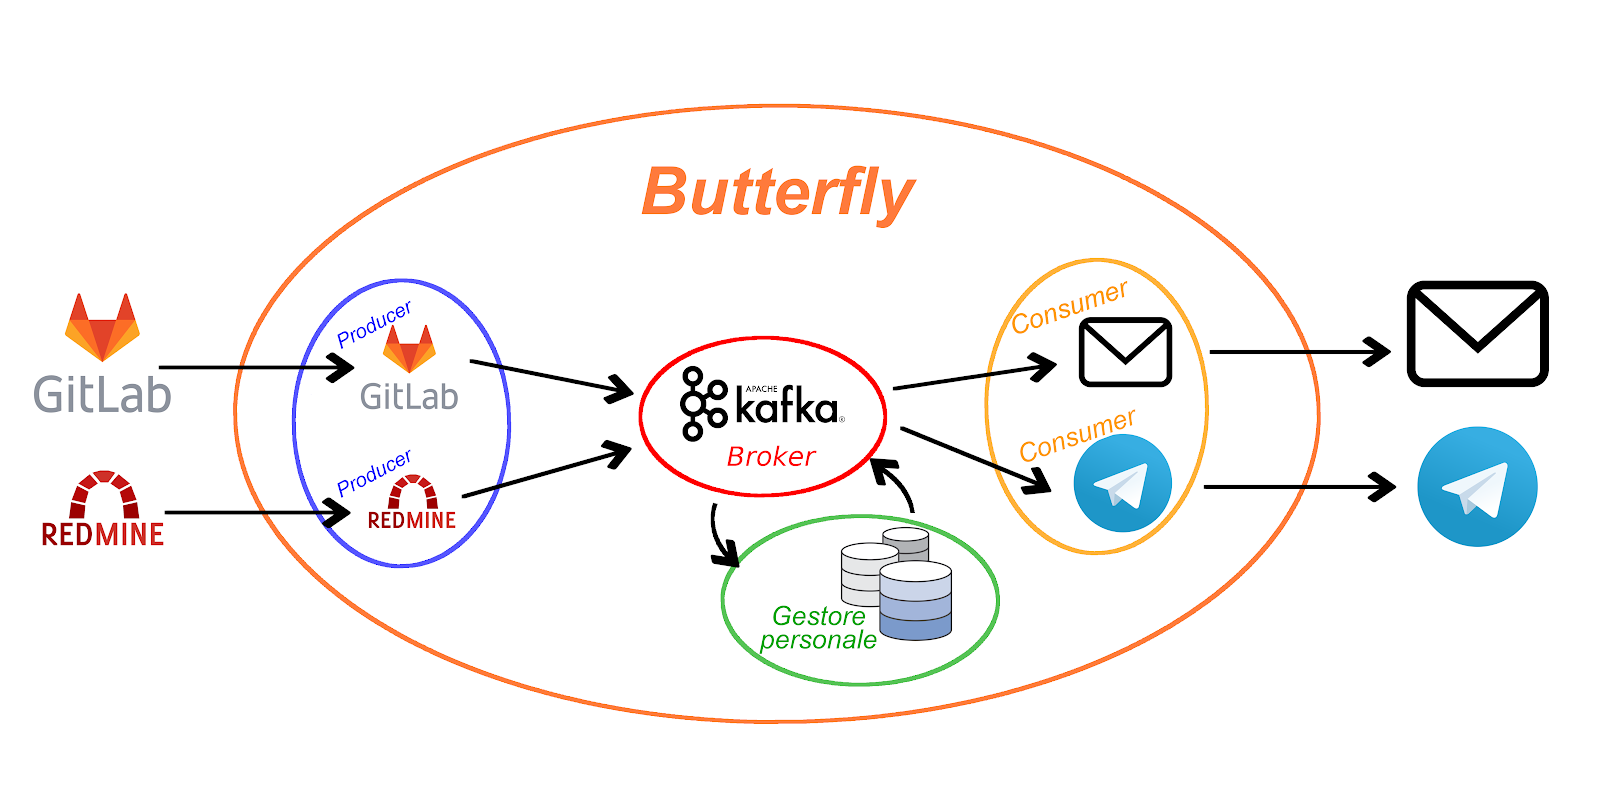
\includegraphics[width=\textwidth]{img/butterfly.png}\\
		\caption{Visione generale del sistema \progetto}
		\label{fig:butterfly}
	\end{figure}
\newpage
	L'immagine precedente rappresenta una suddivisione del sistema in quattro sezioni principali:
	\begin{itemize}
		\item \textbf{Arancione}: \progetto, il sistema nella sua interezza.
		\item \textbf{Blu}: I Producer di GitLab e Redmine.
		\item \textbf{Rosso}: Il Broker. Per \progetto\ useremo Apache Kafka.
		\item \textbf{Verde}: Il Gestore Personale.
		\item \textbf{Giallo}: I Consumer di Telegram ed \mail
	\end{itemize}
	Questa scomposizione ci ha permesso di analizzare più approfonditamente i vari sottosistemi del prodotto in rapporto alle tecnologie esterne a Butterfly (GitLab, Redmine, Telegram ed \mail), ai microservizi interni come i Producer / Consumer associati e il Broker.

	\subsubsection{Producer}\label{TecnologieProducer}

		Per ciascuno degli strumenti che invia messaggi verso il sistema è necessario creare una componente applicativa di tipo Producer che li riceva e li elabori inoltrandoli successivamente verso il Broker.
		Le tecnologie dalle quali vengono ricevuti i messaggi sono elencate di seguito in ordine di priorità in base a quanto richiesto dalla \gloss{proponente}.
		\begin{enumerate}
			\item Redmine
			\item GitLab
			\item SonarQube
		\end{enumerate}
		Abbiamo scelto di sviluppare i Producer per le prime due applicazioni in base alle priorità suggerite da \II\ nel capitolato, lasciando l'applicativo relativo a SonarQube come opzionale.
		Ciascun messaggio ricevuto da queste tecnologie verrà analizzato dal Producer associato in modo da inserirli nel Topic appropriato.

		\paragraph{Producer GitLab}
		Gli eventi relativi alle \gloss{repository} di GitLab presi in considerazione sono:
		\begin{itemize}
			\item Push
			\item \gloss{Issue}, che verranno suddivisi in:
			\begin{itemize}
				\item Apertura issue
				\item Chiusura issue
			\end{itemize}
		\end{itemize}
		Le segnalazioni sono generate in base alle \gloss{keyword} contenute nei messaggi di commit e nelle etichette assegnate alle issue.
		Da quest'ultime verrà creato il Topic corrispondente in caso non sia già esistente.

		\paragraph{Producer Redmine}
		Gli eventi relativi ai progetti di Redmine presi in considerazione, sono:
		\begin{itemize}
			\item Issue, che verranno suddivisi in:
			\begin{itemize}
				\item Apertura issue
				\item Chiusura issue
			\end{itemize}
		\end{itemize}


%		\subsubsection{SonarQube}
%		Come GitLab, anche SonarQube prevede l'utilizzo di Webhooks\footnote{\url{https://docs.sonarqube.org/latest/project-administration/Webhooks/}} che dopo ciascuna build comunica il risultato e le informazioni relative ad essa ad un microservizio capace di aggiornare i dati presenti nel gestore personale e, anche in questo caso, inoltrare le notifiche ai customer interessati.

	\subsubsection{Apache Kafka}\label{TecnologieBroker}
	Il ruolo di Apache Kafka è quello di restare in ascolto dei messaggi provenienti dai
	Producer, e smistarli in determinati Topic, in base al contenuto degli stessi.
	Il Gestore Personale potrà poi reperire i messaggi dai Topic specifici e,
	in base ai Topic ai quali gli utenti sono abbonati, immettere quei messaggi rielaborati alle code specifiche del Broker relative ai Consumer, che si occuperanno di
	inoltrare il messaggio all'utente finale.

		% Il ruolo del Broker è quello di smistare i messaggi in base ai Topic con cui questi sono contrassegnati verso i vari microservizi con cui l'utente ha deciso che gli venga inoltrata la notifica.
		% L'azienda ci consiglia di utilizzare come Broker per i messaggi \gloss{Apache Kafka}.

	\subsubsection{Consumer}\label{TecnologieConsumer}
		Come per gli strumenti precedentemente elencati, anche per quelli su cui il messaggio andrà ad essere inoltrato, è necessaria la creazione di un microservizio in grado di fare da tramite tra Broker e \gloss{client} dello strumento di messaggistica scelto dall'utente.
		Le tecnologie verso le quali vengono inoltrati i messaggi rielaborati dal sistema sono elencate di seguito in ordine di priorità in base a quanto richiesto dalla proponente.
		\begin{enumerate}
			\item Telegram
			\item \mail
			\item Slack
		\end{enumerate}
		Allo stesso modo dei Producer, abbiamo scelto di sviluppare i Consumer per le prime due applicazioni in base alle priorità suggeriteci da \II\ nel capitolato, lasciando l'applicativo relativo a Slack come opzionale.

		\paragraph{Consumer Telegram}
		Il Consumer Telegram ha il ruolo di restare in ascolto del Topic specifico
		per Telegram di Apache Kafka e, usando come tramite un bot Telegram dedicato, inoltrare i messaggi agli utenti che hanno impostato Telegram come piattaforma di
		messaggistica preferita.

		Questo richiederà uno step aggiuntivo per gli utenti, che dovranno mettersi
		in contatto con il bot la prima volta in modo che quest'ultimo abbia il permesso di inviare
		loro i messaggi tramite la piattaforma.

		\paragraph{Consumer \mail}
		Il Consumer Email ha il ruolo di restare in ascolto del Topic specifico per
		le Email di Apache Kafka e, interfacciandosi con un server e-mail dedicato,
		inoltrare i messaggi agli utenti finali che hanno impostato \mail\ come
		preferenza per la ricezione.
		% Le tecnologie alle quali vengono inoltrati i messaggi sono elencate di seguito in ordine di priorità in base a quanto richiesto dal committente.

		%https://realpython.com/python-send-email/

%		\subsubsection{Slack}
%		È possibile utilizzare le API di Slack per poter mandare push notifications ai canali o alle persone interessate specificando il nome del canale (o lo username della persona), testo del messaggio, e lo username che verrà mostrato per il mittente.
%		%https://www.confluent.io/blog/real-time-syslog-processing-with-apache-kafka-and-ksql-part-2-event-driven-alerting-with-slack/

	\subsubsection{Gestore Personale}\label{TecnologieGestorePersonale}
	Il Gestore Personale è quel \gloss{componente} che permette agli utenti di impostare le
	proprie preferenze e i dati personali tramite interfaccia web, installata in un server
	interno all'azienda.

	Questo è accessibile dai dipendenti interessati, i quali potranno quindi modificare, aggiungere e rimuovere, determinate impostazioni riguardanti le proprie
	preferenze. Quest'ultime sono:
	\begin{itemize}
		\item Scelta dell'applicativo sul quale ricevere le notifiche (Telegram / \mail)
		\item Iscrizione / disiscrizione a determinati Topic
		\item Aggiunta / rimozione di determinate keyword per i commit di GitLab
		\item Selezione dei giorni di calendario in cui l'utente segnala la sua assenza
		\item Aggiunta / rimozione / modifica utenti
	\end{itemize}
%	Nel caso arrivasse una notifica da inoltrare a un utente indisponibile,
%	questa verrà inoltrata alla persona più adatta e disponibile al momento.

%    \paragraph{Informazioni aggiuntive}
%    Di seguito vengono spiegati i motivi di alcune scelte progettuali per il Gestore Personale.
%    \begin{itemize}
%        \item \textbf{Persona di fiducia}: per persona di fiducia s'intende un utente a cui inoltrare le notifiche nel momento in cui non si è disponibili. Nel caso in cui questa non sia disponibile \progetto\ inoltrerà di nuovo il messaggio alla persona di fiducia della persona di fiducia. Per evitare che questo processo causi un cicli infinito dopo n inoltri il messaggio viene perso.
%        \item \textbf{Disiscrizione}: non abbiamo previsto un caso specifico per la disiscrizione, ma questo può avvenire se nella rimozione di un utente l'utilizzatore rimuove se stesso.
%    \end{itemize}

	% \subsubsection{Informazioni preconfigurate}
	% I dati relativi ai profili esistenti degli utenti presenti nel sistema (ovvero l'identificativo) e le keyword da riconoscere all'interno dei messaggi che vengono ricevuti da GitLab / Redmine, sono considerati già esistenti e presenti nel database del Gestore Personale.
	% Questo in quanto non è richiesto da \II\ un sistema di autenticazione, poiché si considera che l'applicativo sia utilizzato internamente all'azienda.
	% Non è nemmeno richiesta una configurazione iniziale delle keyword.
	% Il progetto quindi non si occupa della gestione dei profili utente in maniera completa e nemmeno di fornire le keyword da riconoscere.
	% Per questo motivo non abbiamo pensato a un procedimento di autenticazione tramite la coppia username e password, ma solamente a un identificativo al fine di poter differenziare i diversi utenti.